\section{训练结果}
在训练进行约 100 h 后, Q表逐渐收敛,此时学习鼠行为模式能够适应规则鼠的变化。

图\ref{figure_heatmap}展示了在实验中各阶段机器鼠在$1~min$内的活动区域及运动轨迹,阶段划分标准为:
\begin{enumerate}[leftmargin=0em, listparindent=2em, parsep=0em, topsep=0em, label=(\theenumi)]
%\setlength{\leftmargin}{0em}
\setlength{\itemindent}{4em}
\setlength{\labelsep}{0em}
\setlength{\labelwidth}{2em}
\setlength{\parsep}{0em}
\setlength{\itemsep}{0em}
\setlength{\topsep}{0em}
%\setlength{\listparindent}{2em}
  \item 初期:实验启动期,迭代次数$<1000$,Q表中至少有一处状态-动作组合对应的值未完成更新,即保持初始值0。这一阶段大约在实验启动后的$10~min$内结束。
  \item 中期:$1000<$迭代次数$<10000$,Q表全部状态-动作组合对应的值完成了至少一次更新,即学习鼠已经对所有动作进行了尝试。
  \item 后期:迭代次数$>10000$,Q表趋于收敛,经过实验,这一阶段通常为训练$13~h$之后。
\end{enumerate}
\begin{figure}[htbp]
  %\vspace{13pt}
  \centering
  \subfigure[初期]{\label{figure_heatmap_start}
  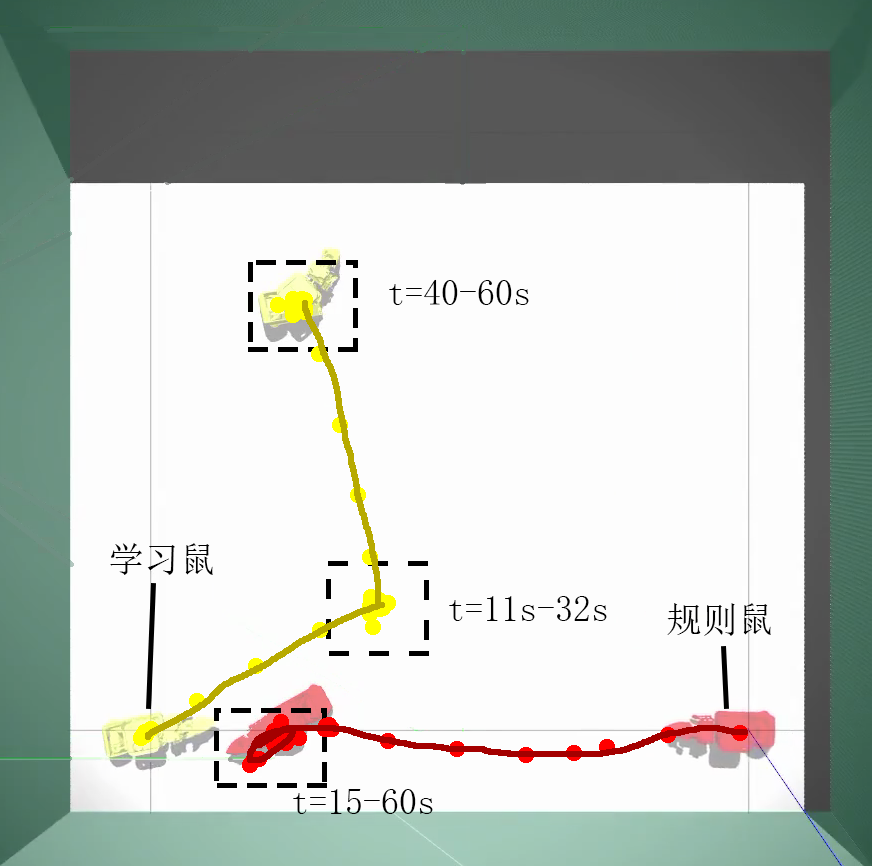
\includegraphics[height=4.5cm]{images/ch05/start/robotic/robotic.png}
  }
  \subfigure[中期]{\label{figure_heatmap_midterm}
  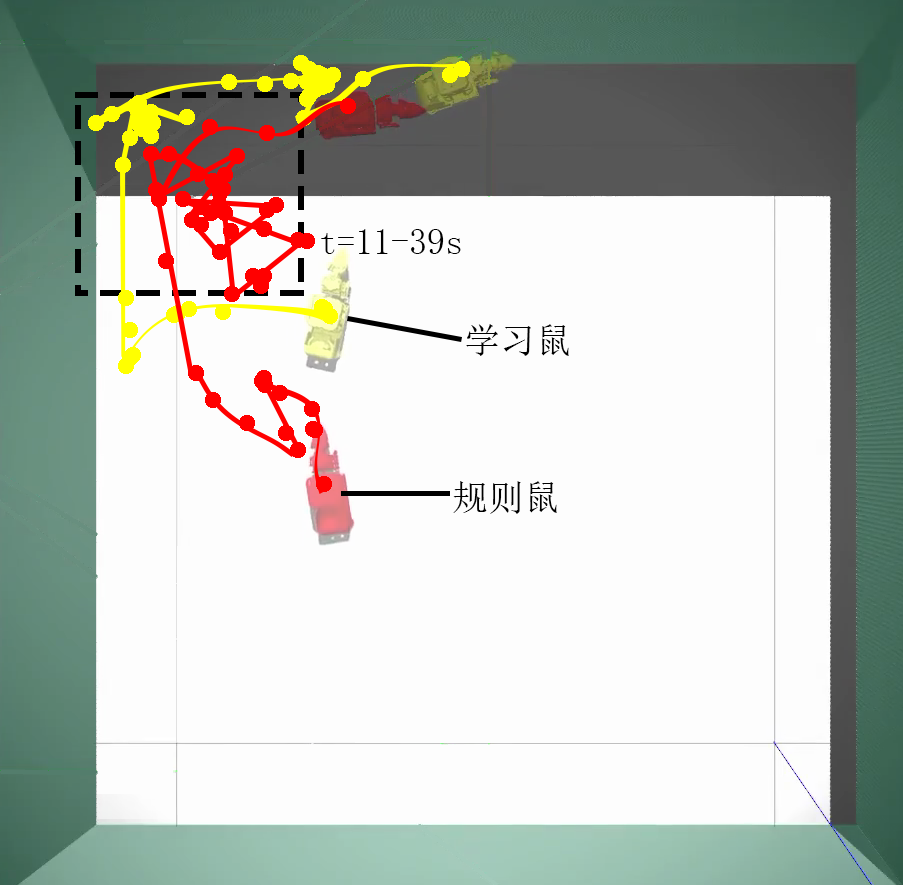
\includegraphics[height=4.5cm]{images/ch05/midterm/heatmap.png}
  }
  \subfigure[后期]{\label{figure_heatmap_end}
  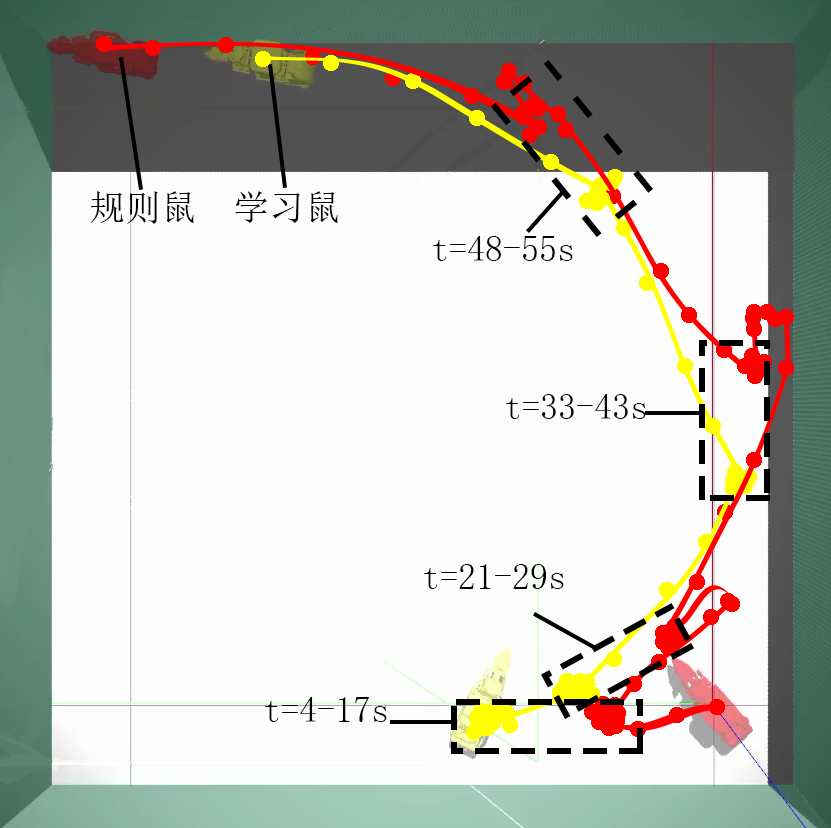
\includegraphics[height=4.5cm]{images/ch05/mature/heatmap.png}
  }
  \caption{实验各阶段机器鼠活动区域热点图及运动轨迹}\label{figure_heatmap}
\end{figure}

% 在学习鼠开始学习与行为交互相关的知识时,Q表均为其初始值0。这意味着其全部状态-动作组均需进行尝试,难以与规则鼠进行有效的行为交互。而从实际表现看,此阶段学习鼠的行为表现具有极大的随机性,运动方向和动作模式均与生物鼠表现存在较大差异,未能成功引发与规则鼠的交互行为。

% 从图\ref{figure_heatmap}\subref{figure_heatmap_start}中可以看出,在训练初期,$0\sim15~s$内,规则鼠向学习鼠靠拢,尝试与学习鼠进行行为交互,但这一时期学习鼠并未习得任何行为交互的知识,处于完全的“探索”阶段,其动作序列随机生成,因此并未回应规则鼠的这一尝试交互的举动。随后,在$15\sim60~s$内,规则鼠陷入了较长时间“不交互”的状态。

% 学习鼠在这一阶段存在两处停留时间较长的地点,这期间进行了一系列动作尝试。在$11\sim32~s$和$40\sim60~s$这两个时间段内,学习鼠在原地进行了多次方向调整,同时产生了包括被梳理、梳理和攀爬等动作(图\ref{figure_startdirectionchange})。但这些尝试并未引起规则鼠的交互反应,未能达到友好交互的状态。
% \begin{figure}[htbp]
%   %\vspace{13pt}
%   \centering
%   \subfigure[$t=11~s$]{\label{figure_startdirectionchange11}
%   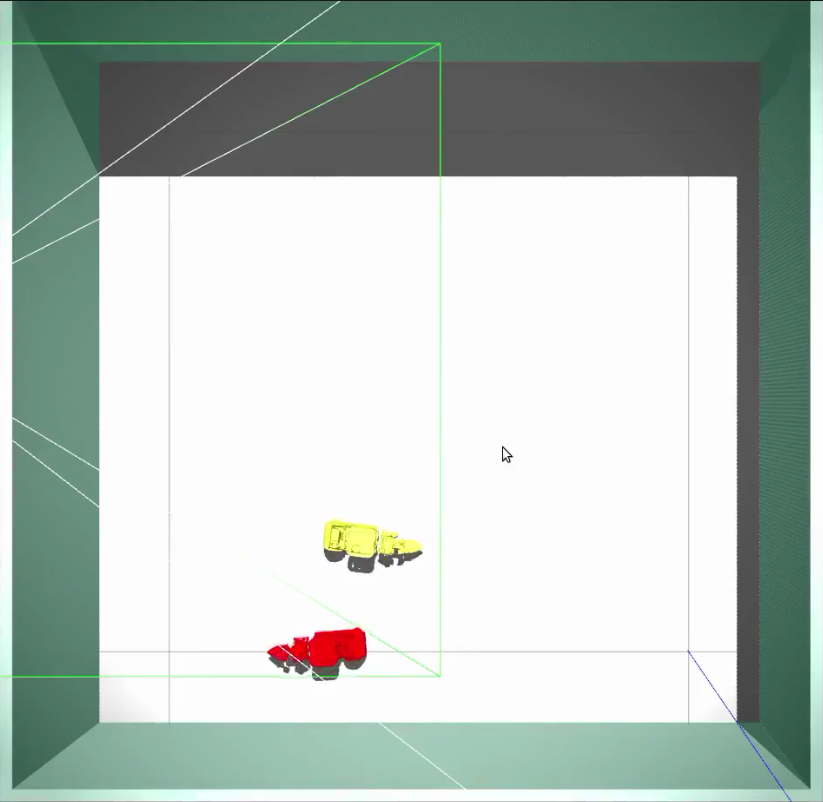
\includegraphics[height=3.9cm]{images/ch05/start/t11.png}
%   }
%   \subfigure[$t=20~s$]{\label{figure_startdirectionchange20}
%   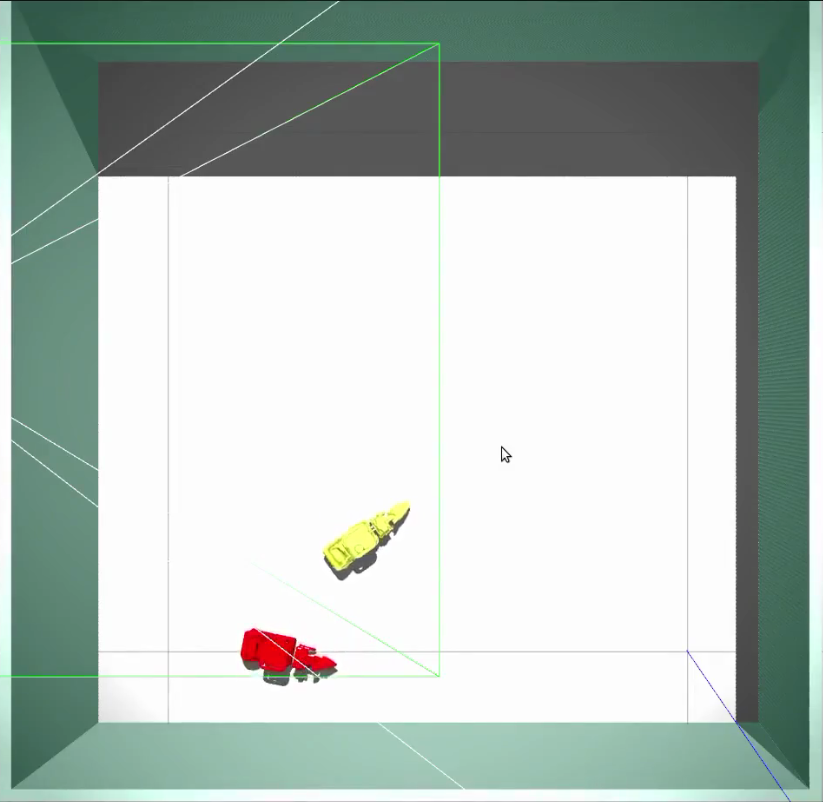
\includegraphics[height=3.9cm]{images/ch05/start/t20.png}
%   }
%   \subfigure[$t=31~s$]{\label{figure_startdirectionchange31}
%   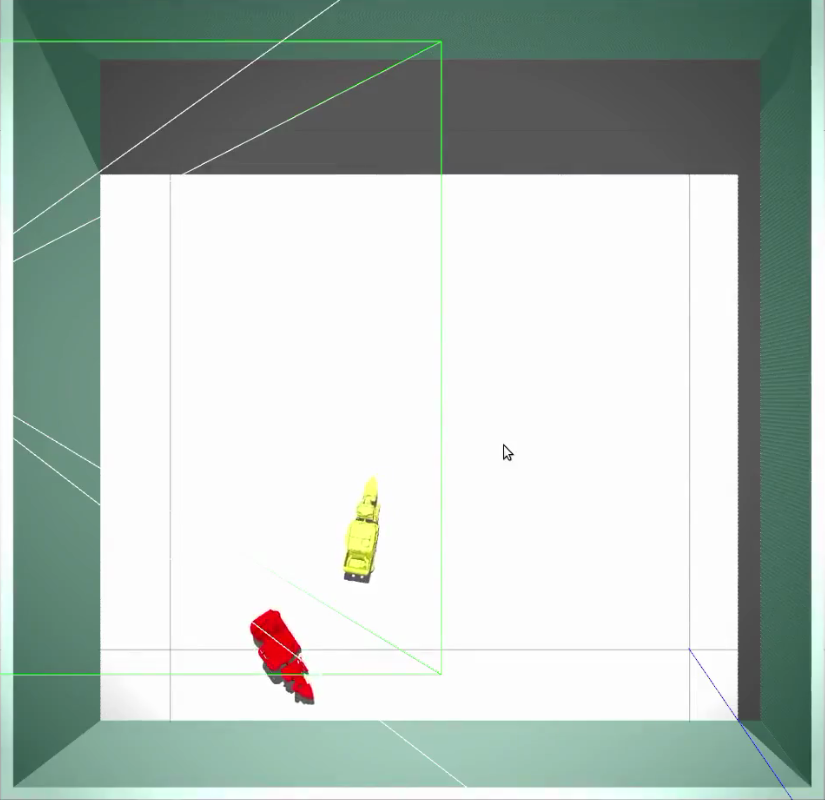
\includegraphics[height=3.9cm]{images/ch05/start/t31.png}
%   }\\
%   \subfigure[$t=42~s$,被梳理]{\label{figure_actionchange42}
%   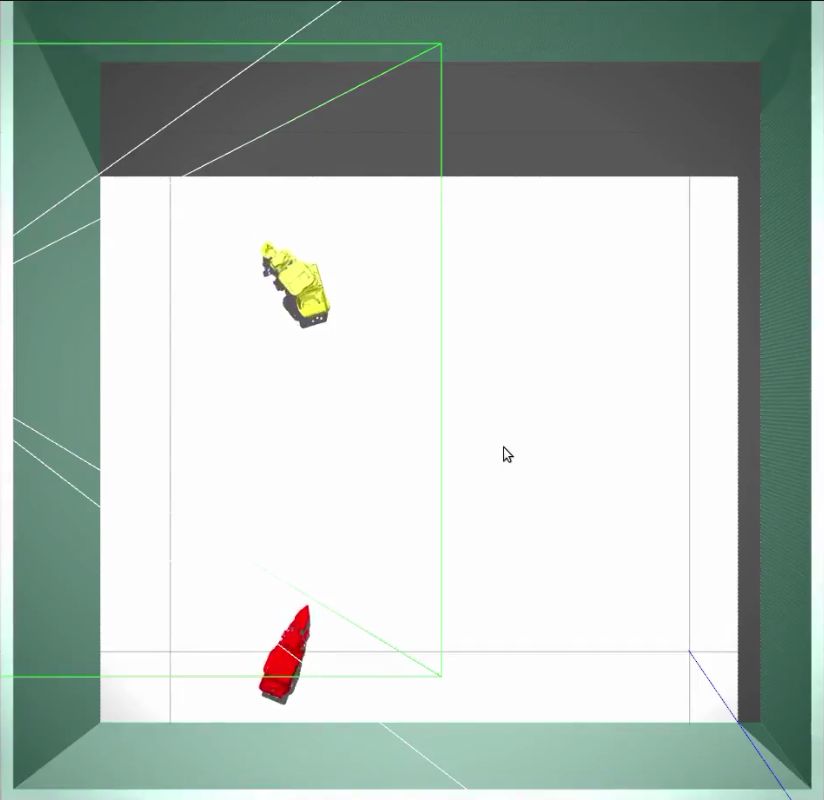
\includegraphics[height=3.9cm]{images/ch05/start/t42.png}
%   }
%   \subfigure[$t=52~s$,梳理]{\label{figure_actionchange52}
%   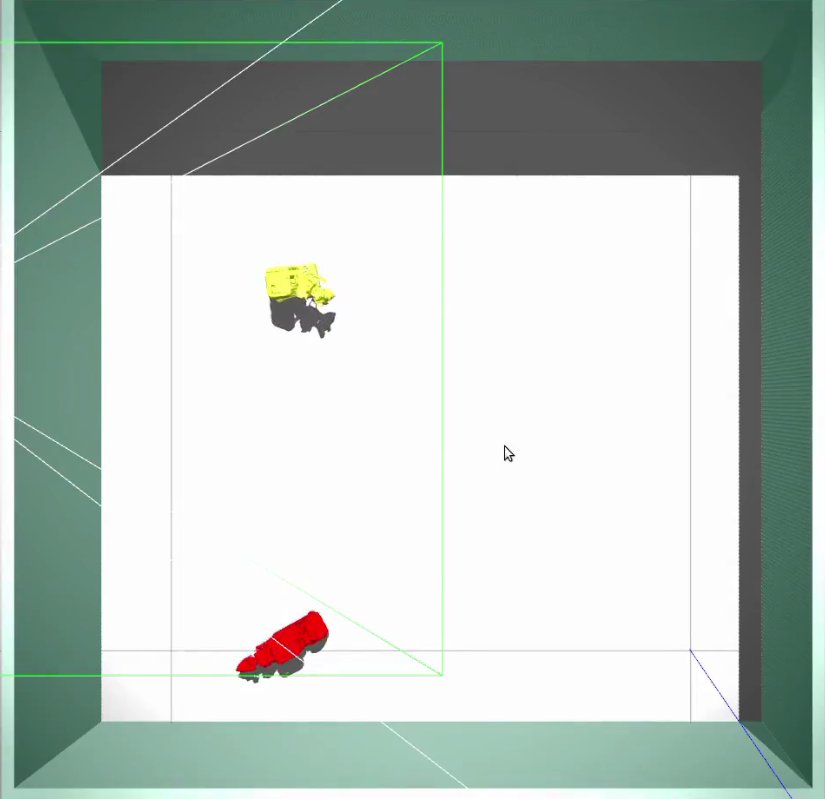
\includegraphics[height=3.9cm]{images/ch05/start/t52.png}
%   }
%   \subfigure[$t=56~s$,攀爬]{\label{figure_actionchange56}
%   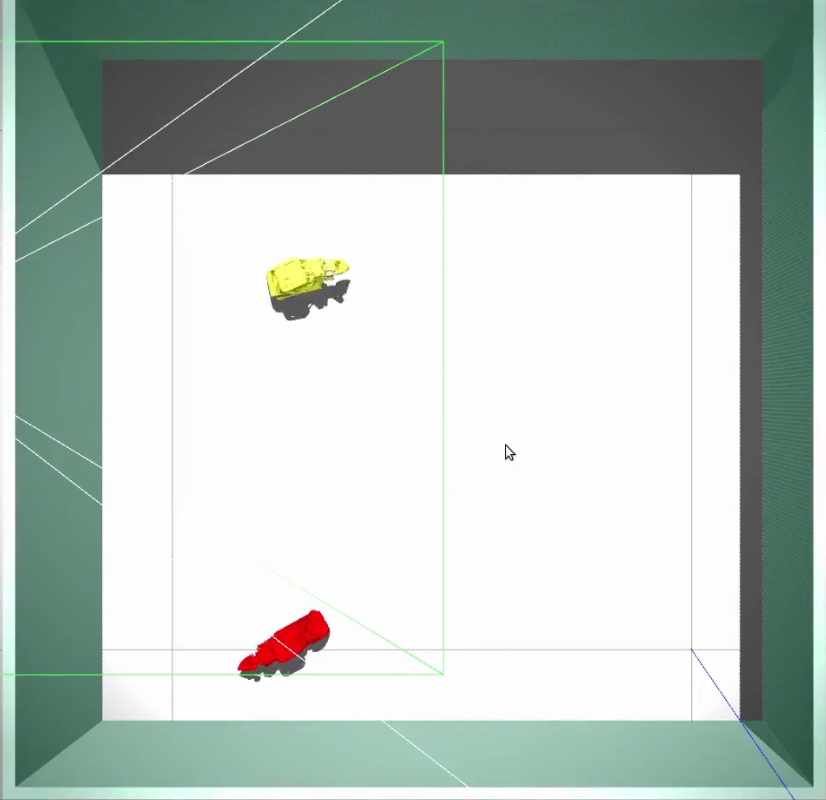
\includegraphics[height=3.9cm]{images/ch05/start/t56.png}
%   }
%   \caption{训练开始阶段学习鼠的动作尝试}\label{figure_startdirectionchange}
% \end{figure}

% 当训练进入中期后,学习鼠更加“活跃”,能够较频繁地改变自身位置,并与机器鼠活动更加一致,例如,在图中的$11\sim39~s$内,两者均在同一角落附加活动,并能够逐渐进行部分行为交互。

% 但即便两者距离足够近,也并不意味着能够开展有效的行为交互。以图\ref{figure_heatmap}\subref{figure_heatmap_midterm}中$35\sim39~s$这一时间段为例,如图\ref{figure_mid35-39}所示,规则鼠始终在学习鼠右侧活动,此时学习鼠虽然产生了梳理等一些试图交互的动作,但由于并未面对交互伙伴,因此规则鼠并未作出回应,只是在不断地靠近和远离学习鼠中切换。
% \begin{figure}[htb]
%   %\vspace{13pt}
%   \centering
%   \subfigure[$t=35~s$]{\label{figure_midt69}
%   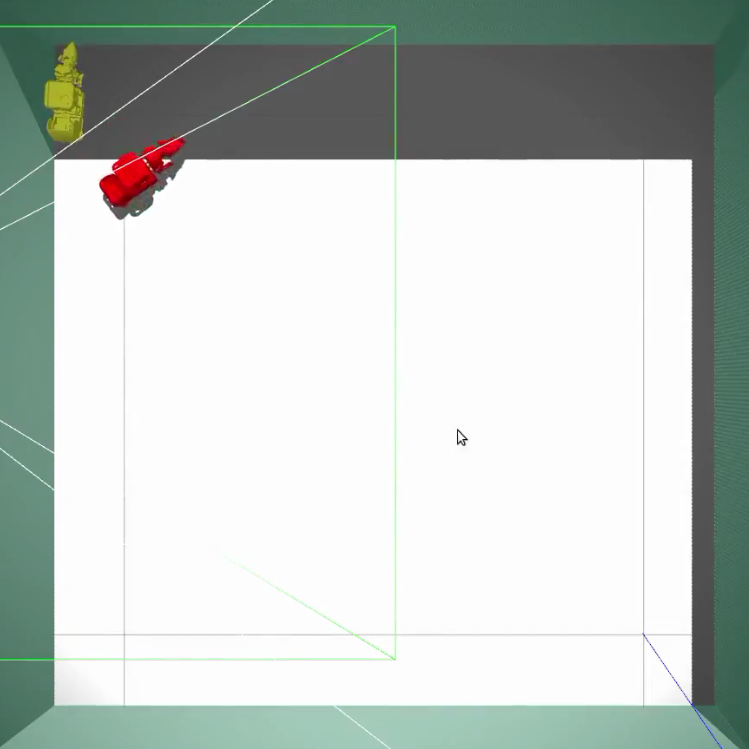
\includegraphics[height=3.5cm]{images/ch05/midterm/t69.png}
%   }
%   \subfigure[$t=36~s$]{\label{figure_midt72}
%   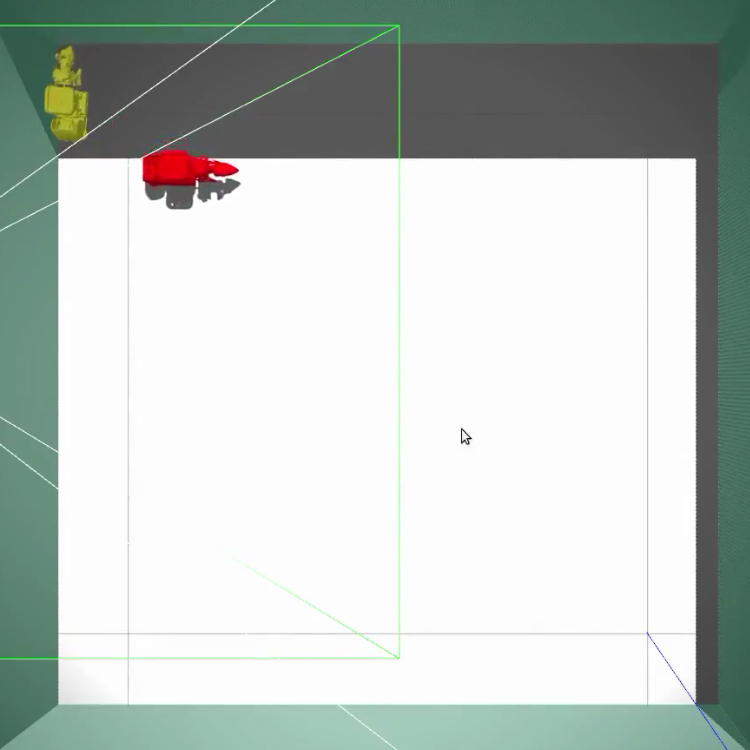
\includegraphics[height=3.5cm]{images/ch05/midterm/t72.png}
%   }
%   \subfigure[$t=37~s$]{\label{figure_midt75}
%   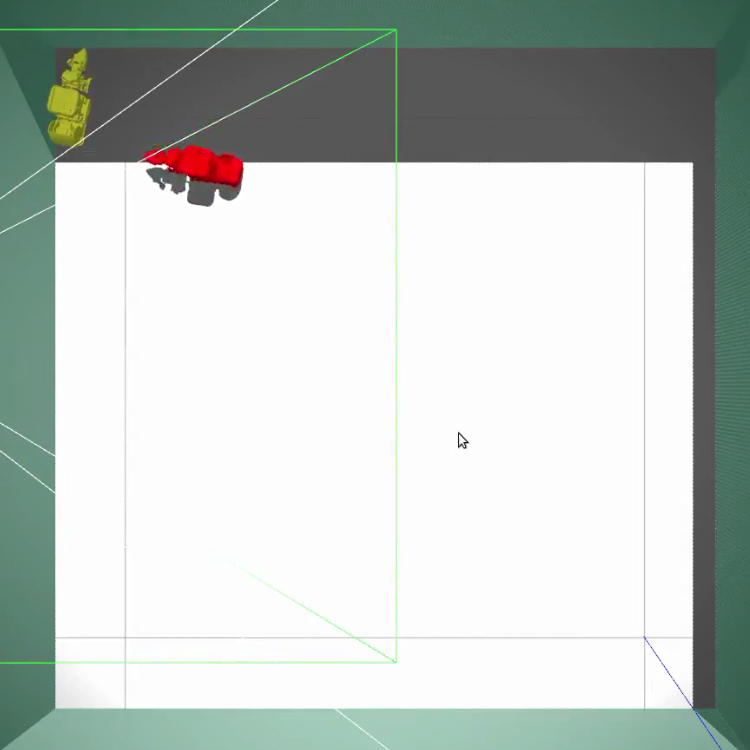
\includegraphics[height=3.5cm]{images/ch05/midterm/t75.png}
%   }
%   \subfigure[$t=38~s$]{\label{figure_midt77}
%   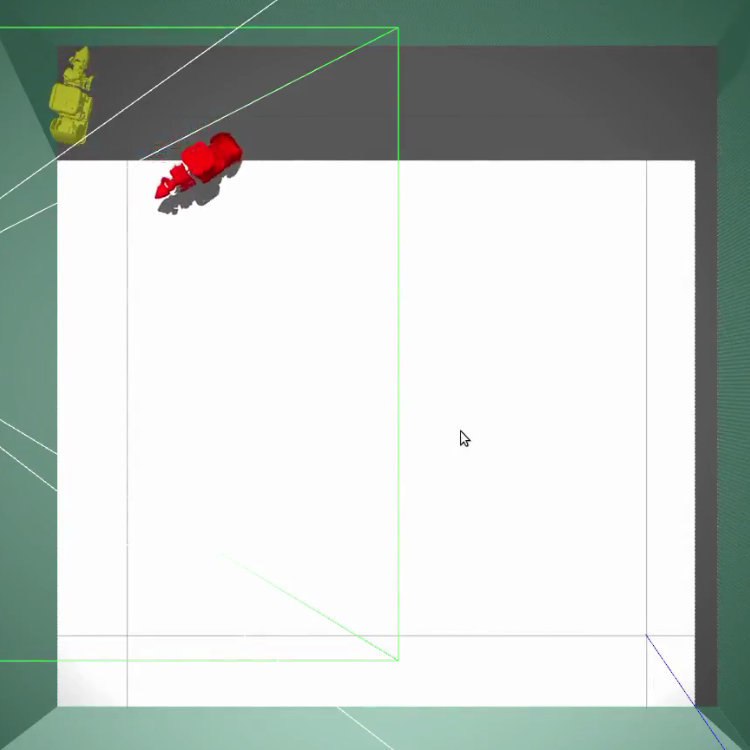
\includegraphics[height=3.5cm]{images/ch05/midterm/t77.png}
%   }
%   \caption{训练中期$35\sim39~s$内学习鼠与规则鼠动作表现($1~min$)}\label{figure_mid35-39}
% \end{figure}

% 这一阶段学习鼠行为的另一特点是试错(trial-and-error search),在图\ref{figure_heatmap}\subref{figure_heatmap_midterm}中,学习鼠长时间停留在墙角便是如此。图\ref{figure_actioncnt}统计了这一时段学习鼠各动作的执行频次,其中浅绿色$s_4$(右转)为理论上其应当执行的最优动作,数据表明这一动作的执行次数明显低于其他动作,而$s_3$(左转)执行次数较多。这是由于前期错误经验的积累,当学习鼠观测到环境处于某一状态时,根据尚不完善的Q表做出错误的决定,因此需要在不断地错误尝试中积累负向奖励,直到这些非最优的状态-动作组Q值低于最优状态-动作组。同样由于强化学习奖励的延时性,负向奖励需要一定时间才能传递到特定状态-动作组,因此试错所需时间较长。
% \begin{figure}[htbp]
%   %\vspace{13pt}
%   \centering
%   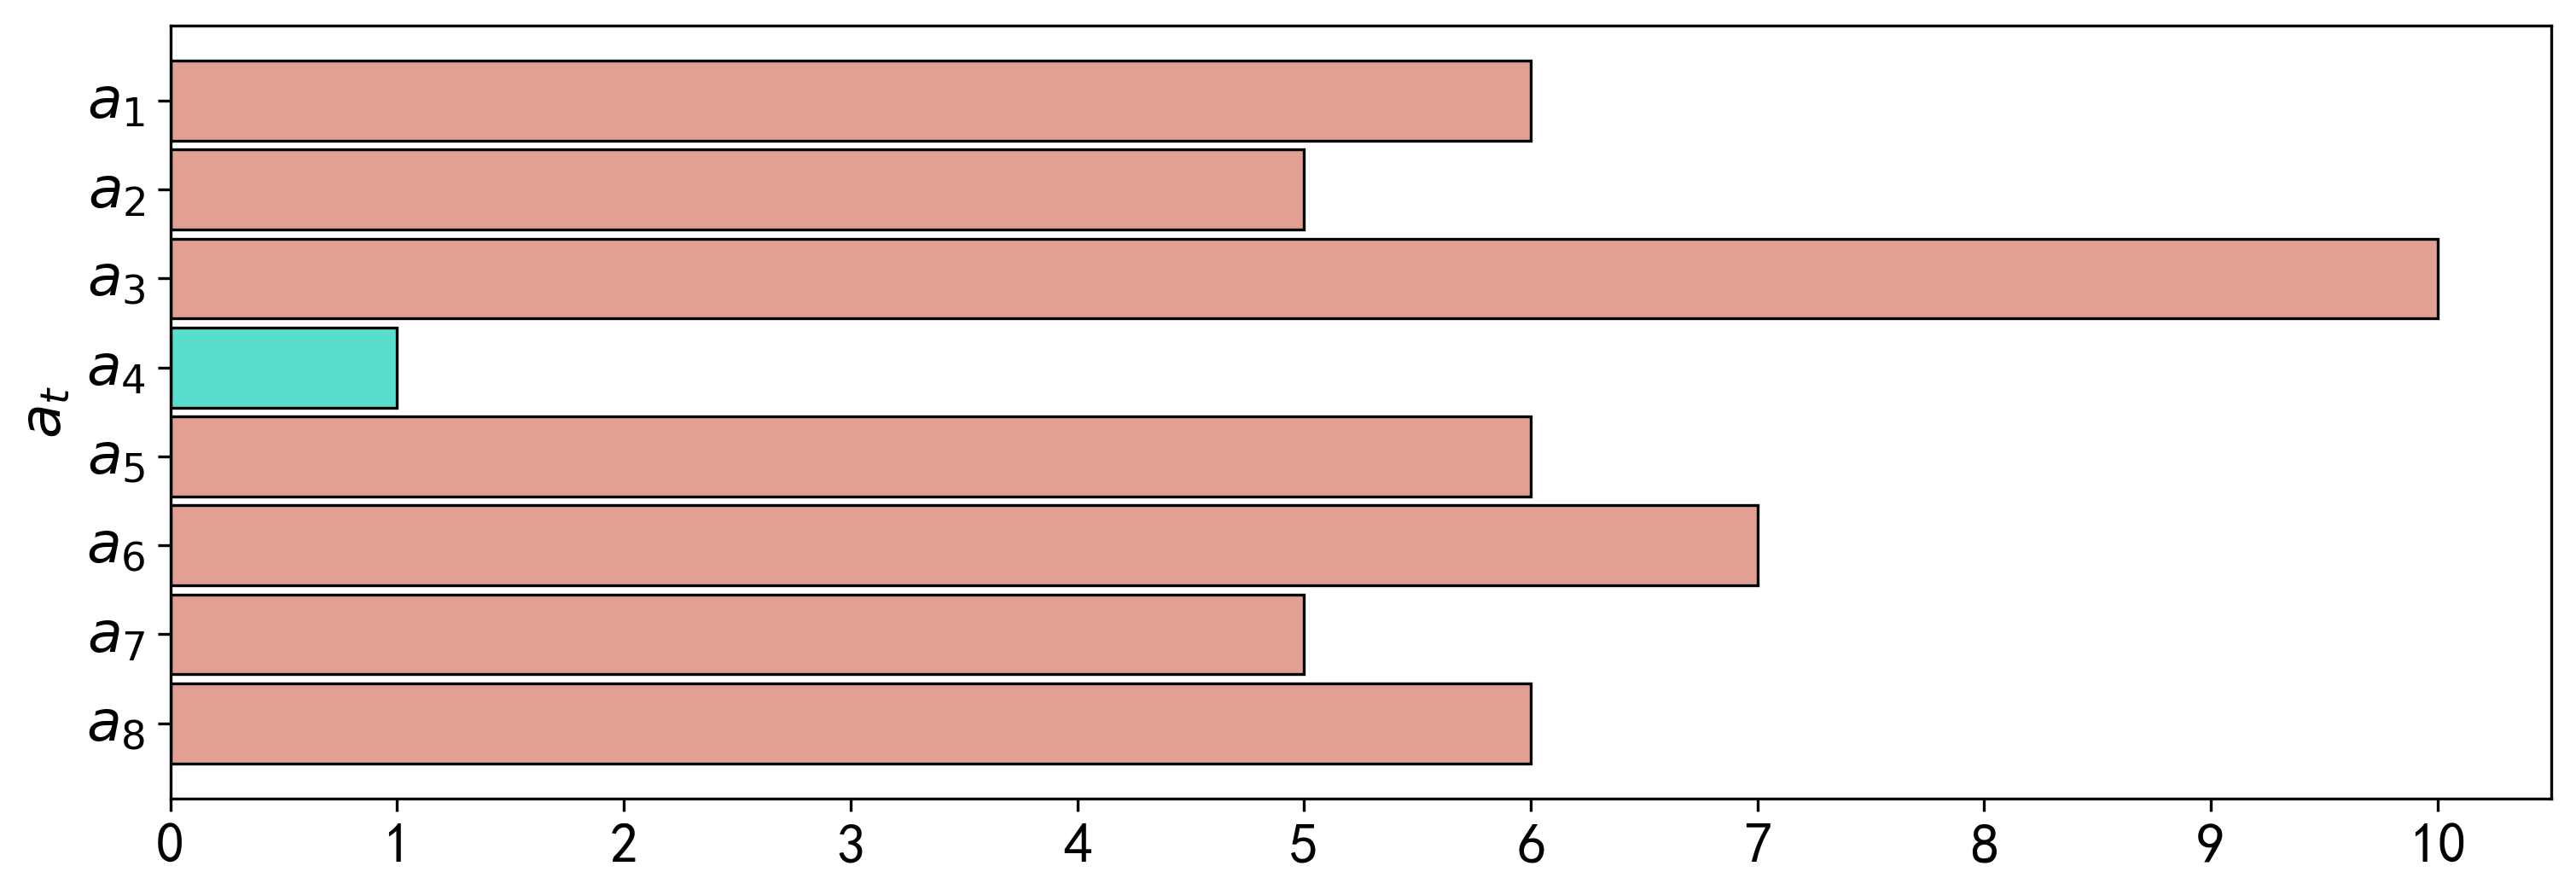
\includegraphics[height=4.5cm]{images/ch05/midterm/actioncnt.png}
%   \caption{训练中期学习鼠在墙角时动作执行频次}\label{figure_actioncnt}
% \end{figure}

% 在训练后期,机器鼠行为表现更加稳定。如图\ref{figure_heatmap}\subref{figure_heatmap_end}所示,规则鼠与学习鼠的活动区域和运动轨迹高度重合。同时,与生物鼠的交互行为(图\ref{figure_livingheatmap})进行对比,
% \begin{figure}[htb]
%   %\vspace{13pt}
%   \centering
%   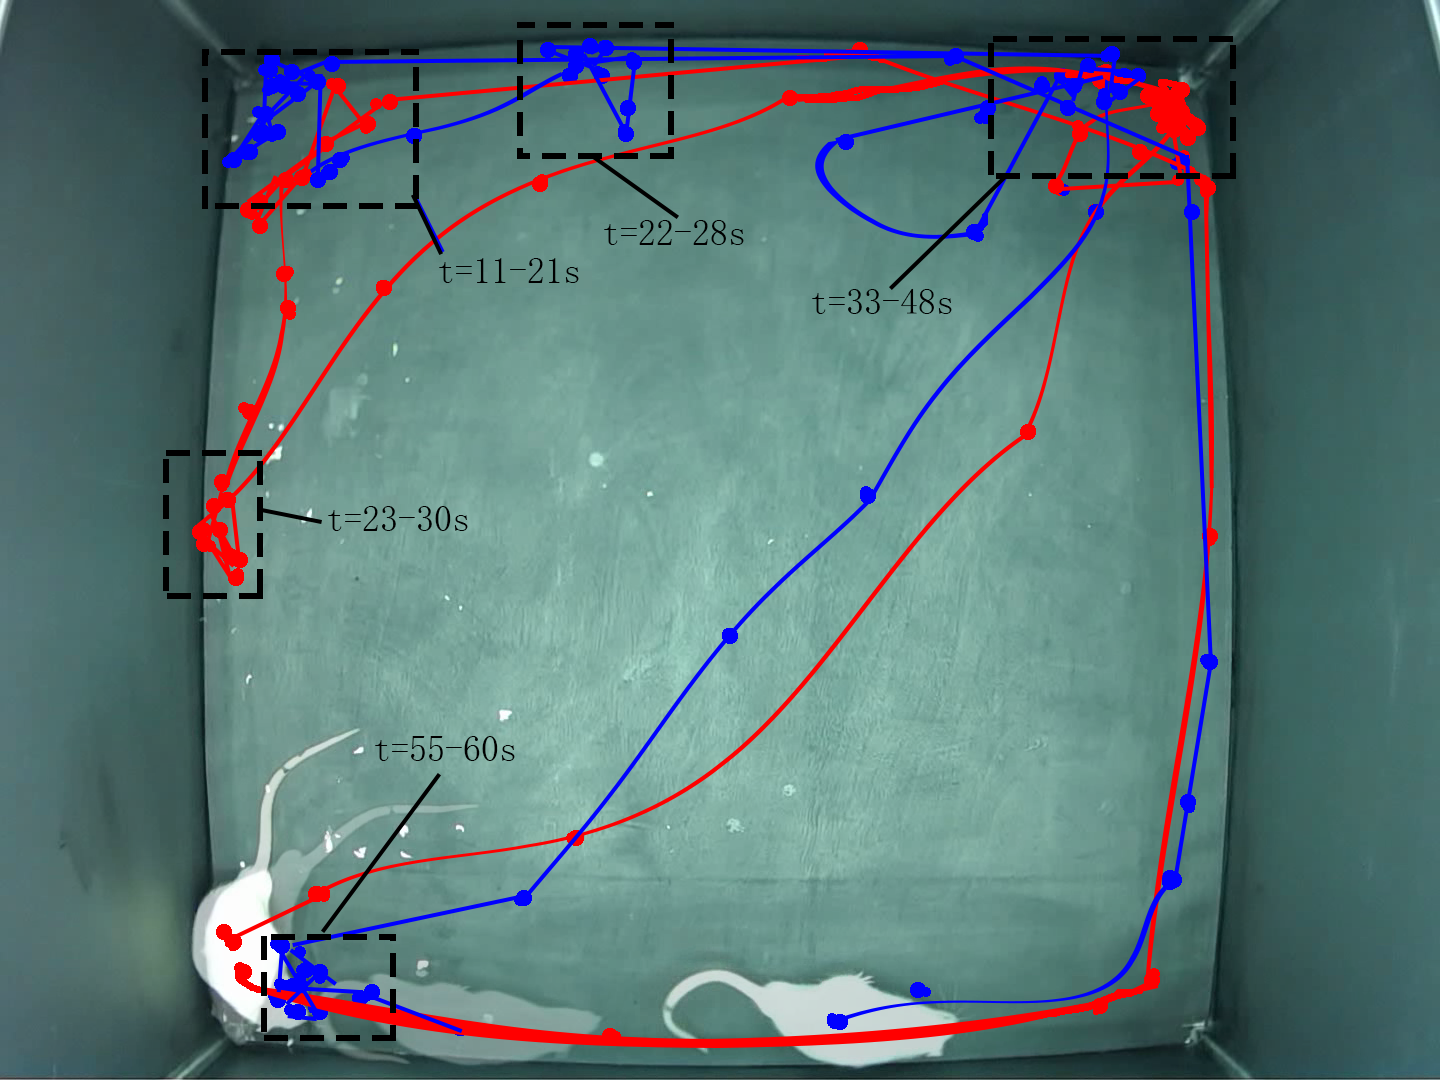
\includegraphics[height=5.5cm]{images/ch05/mature/livingheatmap.png}
%   \caption{生物鼠运动热点图及运动轨迹($1~min$)}\label{figure_livingheatmap}
% \end{figure}
% 可以发现仿生机器鼠在跟随(following)和接近(approaching)等行为模式方面具有相似性。同时,虽然经过Q-学习训练成熟的机器鼠在行为模式上与生物鼠具有一定的相似性,即均倾向于接近和跟随交互伙伴。但在运动范围和二者距离等方面,仿生机器鼠的表现与生物鼠存在差异。

% 图\ref{figure_heatmap}\subref{figure_heatmap_end}和图\ref{figure_livingheatmap}中都存在多处机器鼠或生物鼠停留较长的时段,在图\ref{figure_livingheatmap}中,这些时段意味着生物鼠进行了一些友好的交互行为(图\ref{figure_living1537}\subref{figure_living15}、图\ref{figure_living1537}\subref{figure_living37})。而在图\ref{figure_heatmap}\subref{figure_heatmap_end}中,机器鼠也产生了相似的行为(图\ref{figure_living1537}\subref{figure_matureallow}、图\ref{figure_living1537}\subref{figure_maturecon})。
% \begin{figure}[htb]
%   %\vspace{13pt}
%   \centering
%   \subfigure[$t=15~s$,征服]{\label{figure_living15}
%   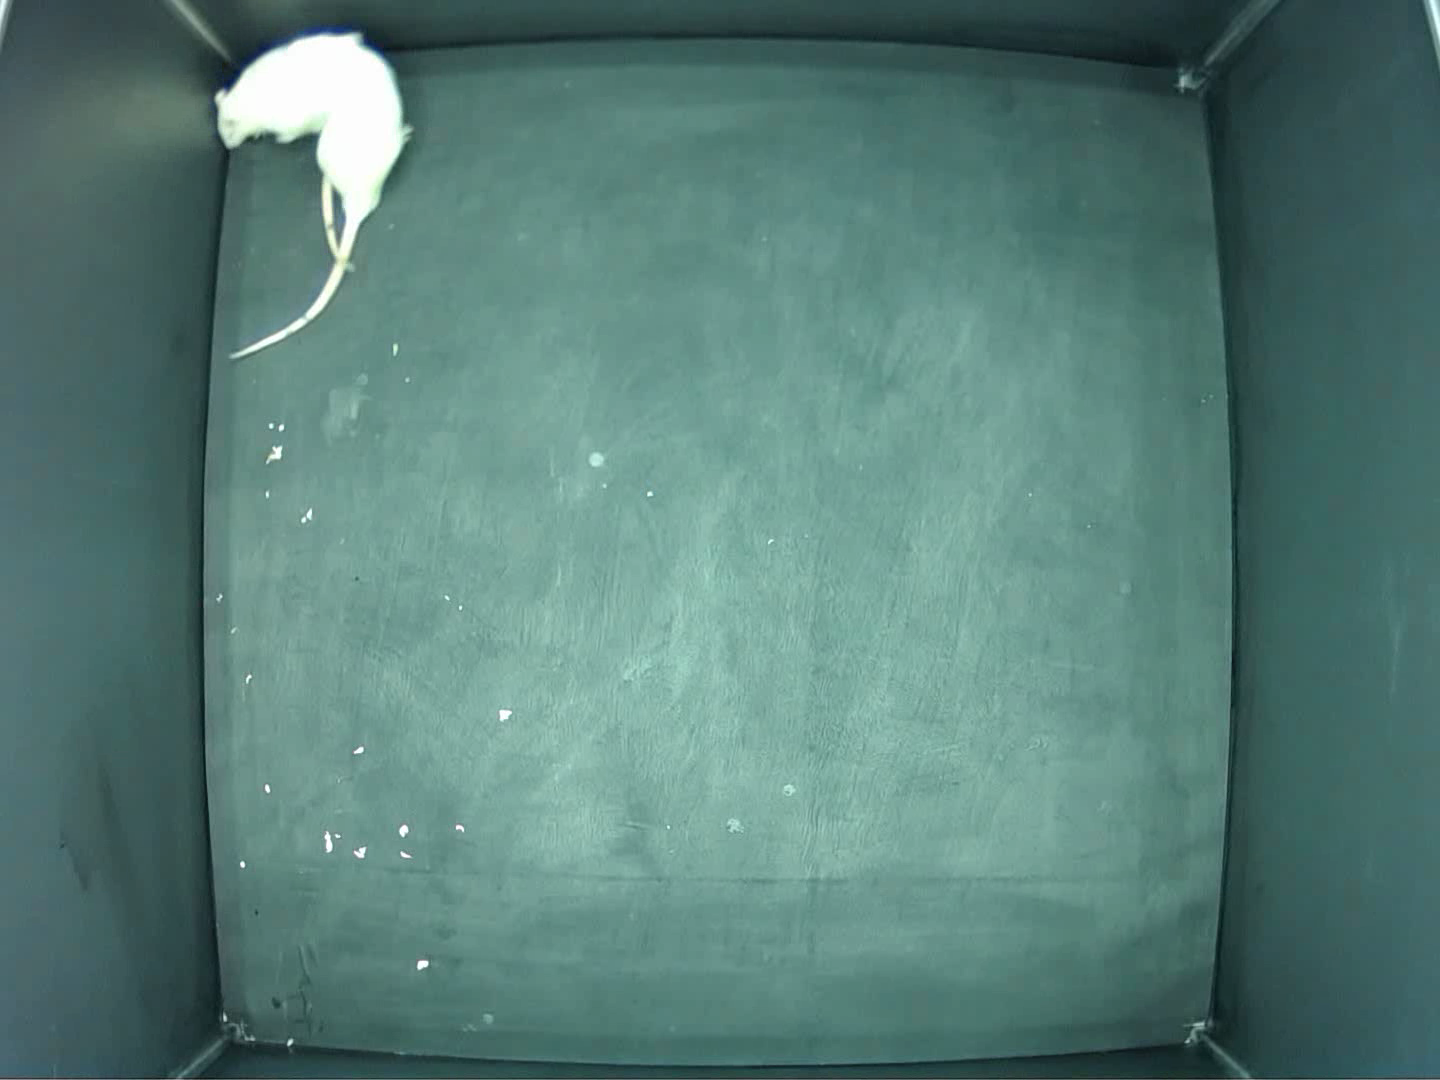
\includegraphics[height=2.7cm]{images/ch05/mature/living15.png}
%   }
%   \subfigure[$t=37~s$,嗅探]{\label{figure_living37}
%   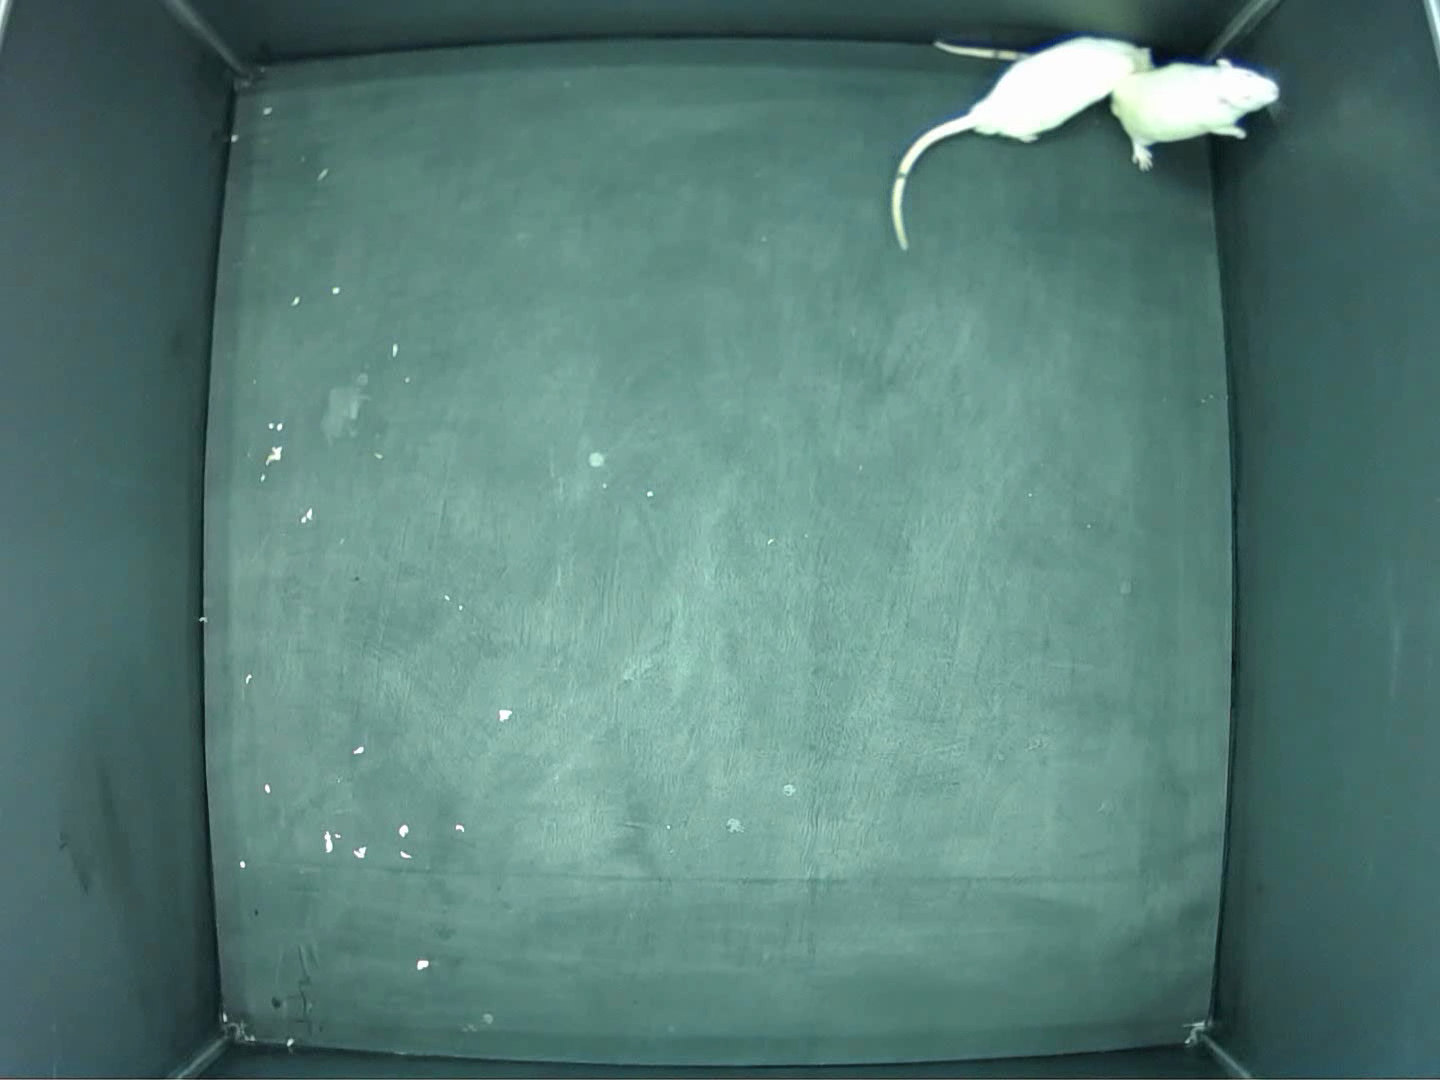
\includegraphics[height=2.7cm]{images/ch05/mature/living37.png}
%   }\hspace{10pt}
%   \subfigure[$t=5~s$,梳理]{\label{figure_matureallow}
%   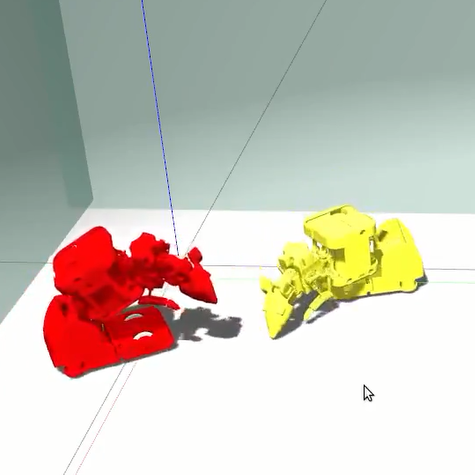
\includegraphics[height=2.7cm]{images/ch05/mature/allow.png}
%   }
%   \subfigure[$t=15~s$,征服]{\label{figure_maturecon}
%   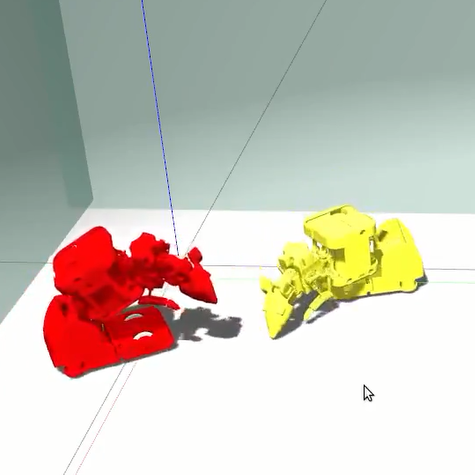
\includegraphics[height=2.7cm]{images/ch05/mature/allow.png}
%   }
%   \caption{生物鼠和机器鼠的交互行为}\label{figure_living1537}
% \end{figure} 